% !TeX root = main.tex
\documentclass[british]{article}
\usepackage[utf8]{inputenc}
\usepackage{amsmath}
\usepackage{mathtools}
\usepackage[margin=1.5cm]{geometry}
\usepackage{float}
\usepackage{listings}
\usepackage{hyperref}
\usepackage{amssymb}
\usepackage{enumerate}
\usepackage[shortlabels]{enumitem}
\usepackage{subcaption}
\usepackage{xr}
\usepackage{graphicx}
\usepackage[demo]{rotating}
\usepackage{wrapfig}
\usepackage{ragged2e}
\usepackage{multicol}
\usepackage{textcomp, gensymb}
\usepackage[useregional]{datetime2}[showzone=false]
\RequirePackage{xkeyval}
\RequirePackage{etoolbox}
\usepackage{csvsimple, booktabs, siunitx}

% Custom configurations and commands
% !TeX root = ..\main.tex
% Custom Commands
\newcommand\dif{\mathop{}\!\mathrm{d}} %dx for integrals \dif{x}
\newcommand\var[1]{\text{Var}\left[\,#1\,\right]} %Var[]
\newcommand\cov[2]{\text{Cov}\left[\,#1,#2\,\right]} %Cov[x1,x2]
\newcommand\E[1]{\text{E}\left[\,#1\,\right]} %E[]
\newcommand\IQR{\text{I}\text{Q}\text{R}}
\newcommand\nline{\par\smallskip}
\newcommand\sOneSize{0.4625}
\newcommand\sTwoRes{0.70}
\newcommand\AR[1]{\text{AR}\left(#1\right)}
\newcommand\MA[1]{\text{MA}\left(#1\right)}
\newcommand\ARMA[2]{\text{ARMA}\left(#1,#2\right)}
\newcommand\ARIMA[3]{\text{ARIMA}\left(#1,#2,#3\right)}
%% Defaults for LstListing Environment
\lstset{
  caption=\lstname,
  basicstyle=\scriptsize\ttfamily, % the size of the fonts that are used for the code
  numbers=left,                   % where to put the line-numbers
  numberstyle=\tiny\color{Black},  % the style that is used for the line-numbers
  stepnumber=1,                   % the step between two line-numbers. If it is 1, each line
                                  % will be numbered
  numbersep=5pt,                  % how far the line-numbers are from the code
  backgroundcolor=\color{white},  % choose the background color. You must add \usepackage{color}
  showspaces=false,               % show spaces adding particular underscores
  showstringspaces=false,         % underline spaces within strings
  showtabs=false,                 % show tabs within strings adding particular underscores
  frame=single,                   % adds a frame around the code
  rulecolor=\color{black},        % if not set, the frame-color may be changed on line-breaks within not-black text (e.g. commens (green here))
  tabsize=2,                      % sets default tabsize to 2 spaces
  captionpos=t,                   % sets the caption-position to top
  breaklines=true,                % sets automatic line breaking
  breakatwhitespace=false,        % sets if automatic breaks should only happen at whitespace
  }
%% Defining Style for R Code within LstListing Environment
\usepackage[usenames,dvipsnames]{color}    
\lstdefinestyle{R}{ 
  language=R,                     % the language of the code
  keywordstyle=\color{RoyalBlue},      % keyword style
  commentstyle=\color{YellowGreen},   % comment style
  stringstyle=\color{ForestGreen}      % string literal style
}
%% Hyperlink customization
\hypersetup{
  %hidelinks    = false, %Remove color box
  frenchlinks  = false, %Small caps for hyperlinks
  colorlinks   = true, %Colours links instead of boxes
  urlcolor     = blue, %Colour for external hyperlinks
  linkcolor    = black, %Colour of internal links
  citecolor   = black   %Colour of citations
}
%% Extra spacing on matrices
\makeatletter
\renewcommand*\env@matrix[1][\arraystretch]{%
  \edef\arraystretch{#1}%
  \hskip -\arraycolsep
  \let\@ifnextchar\new@ifnextchar
  \array{*\c@MaxMatrixCols c}}
\makeatother
\begin{document}
\title{\vspace{-2.0cm}MTHM033 - Statistical Modelling in Space and Time \break 
Assessed Coursework 2}
\author{670033412}
\date{}
\maketitle
% !TeX root = ..\..\main.tex
\vspace{-1.0cm}
\begin{center}
     \Large Strength of Overturning In The North Atlantic
\end{center}
The global overturning of ocean waters involves the equatorward transport of cold, deep waters and the poleward transport of warm, near-surface waters \cite{doi:10.1146/annurev-marine-120710-100740}. Here we use data collected every 12 hours between \DTMshowzonefalse\DTMsettimestyle{iso}\DTMsetdatestyle{iso}\DTMdisplay{2004}{04}{02}{-1}{00}{00}{00}{0}{0} and \DTMdisplay{2014}{03}{22}{-1}{00}{00}{00}{0}{0} from a mooring positioned at $26^\circ$N measured in Sverdrup (Sv) or cubic hectometers per second (hm$^3/$s).
% !TeX root = ..\..\main.tex
\section{Data Integrity}

We begin by first running a summary on the data to ensure that all the values are within the ranges we would expect.

\lstinputlisting[caption={Summary of Data}]{Sections/DataIntegretity/Outputs/summary.txt}

We can see that our data ranges are appropriate for our date and time columns however, without prior knowledge of the range of overturning strength it is difficult to detect outliers. We may attempt to do so using a box plot

\begin{figure}[H]
    \centering
    \begin{subfigure}[b]{\sOneSize\textwidth}
        \centering
        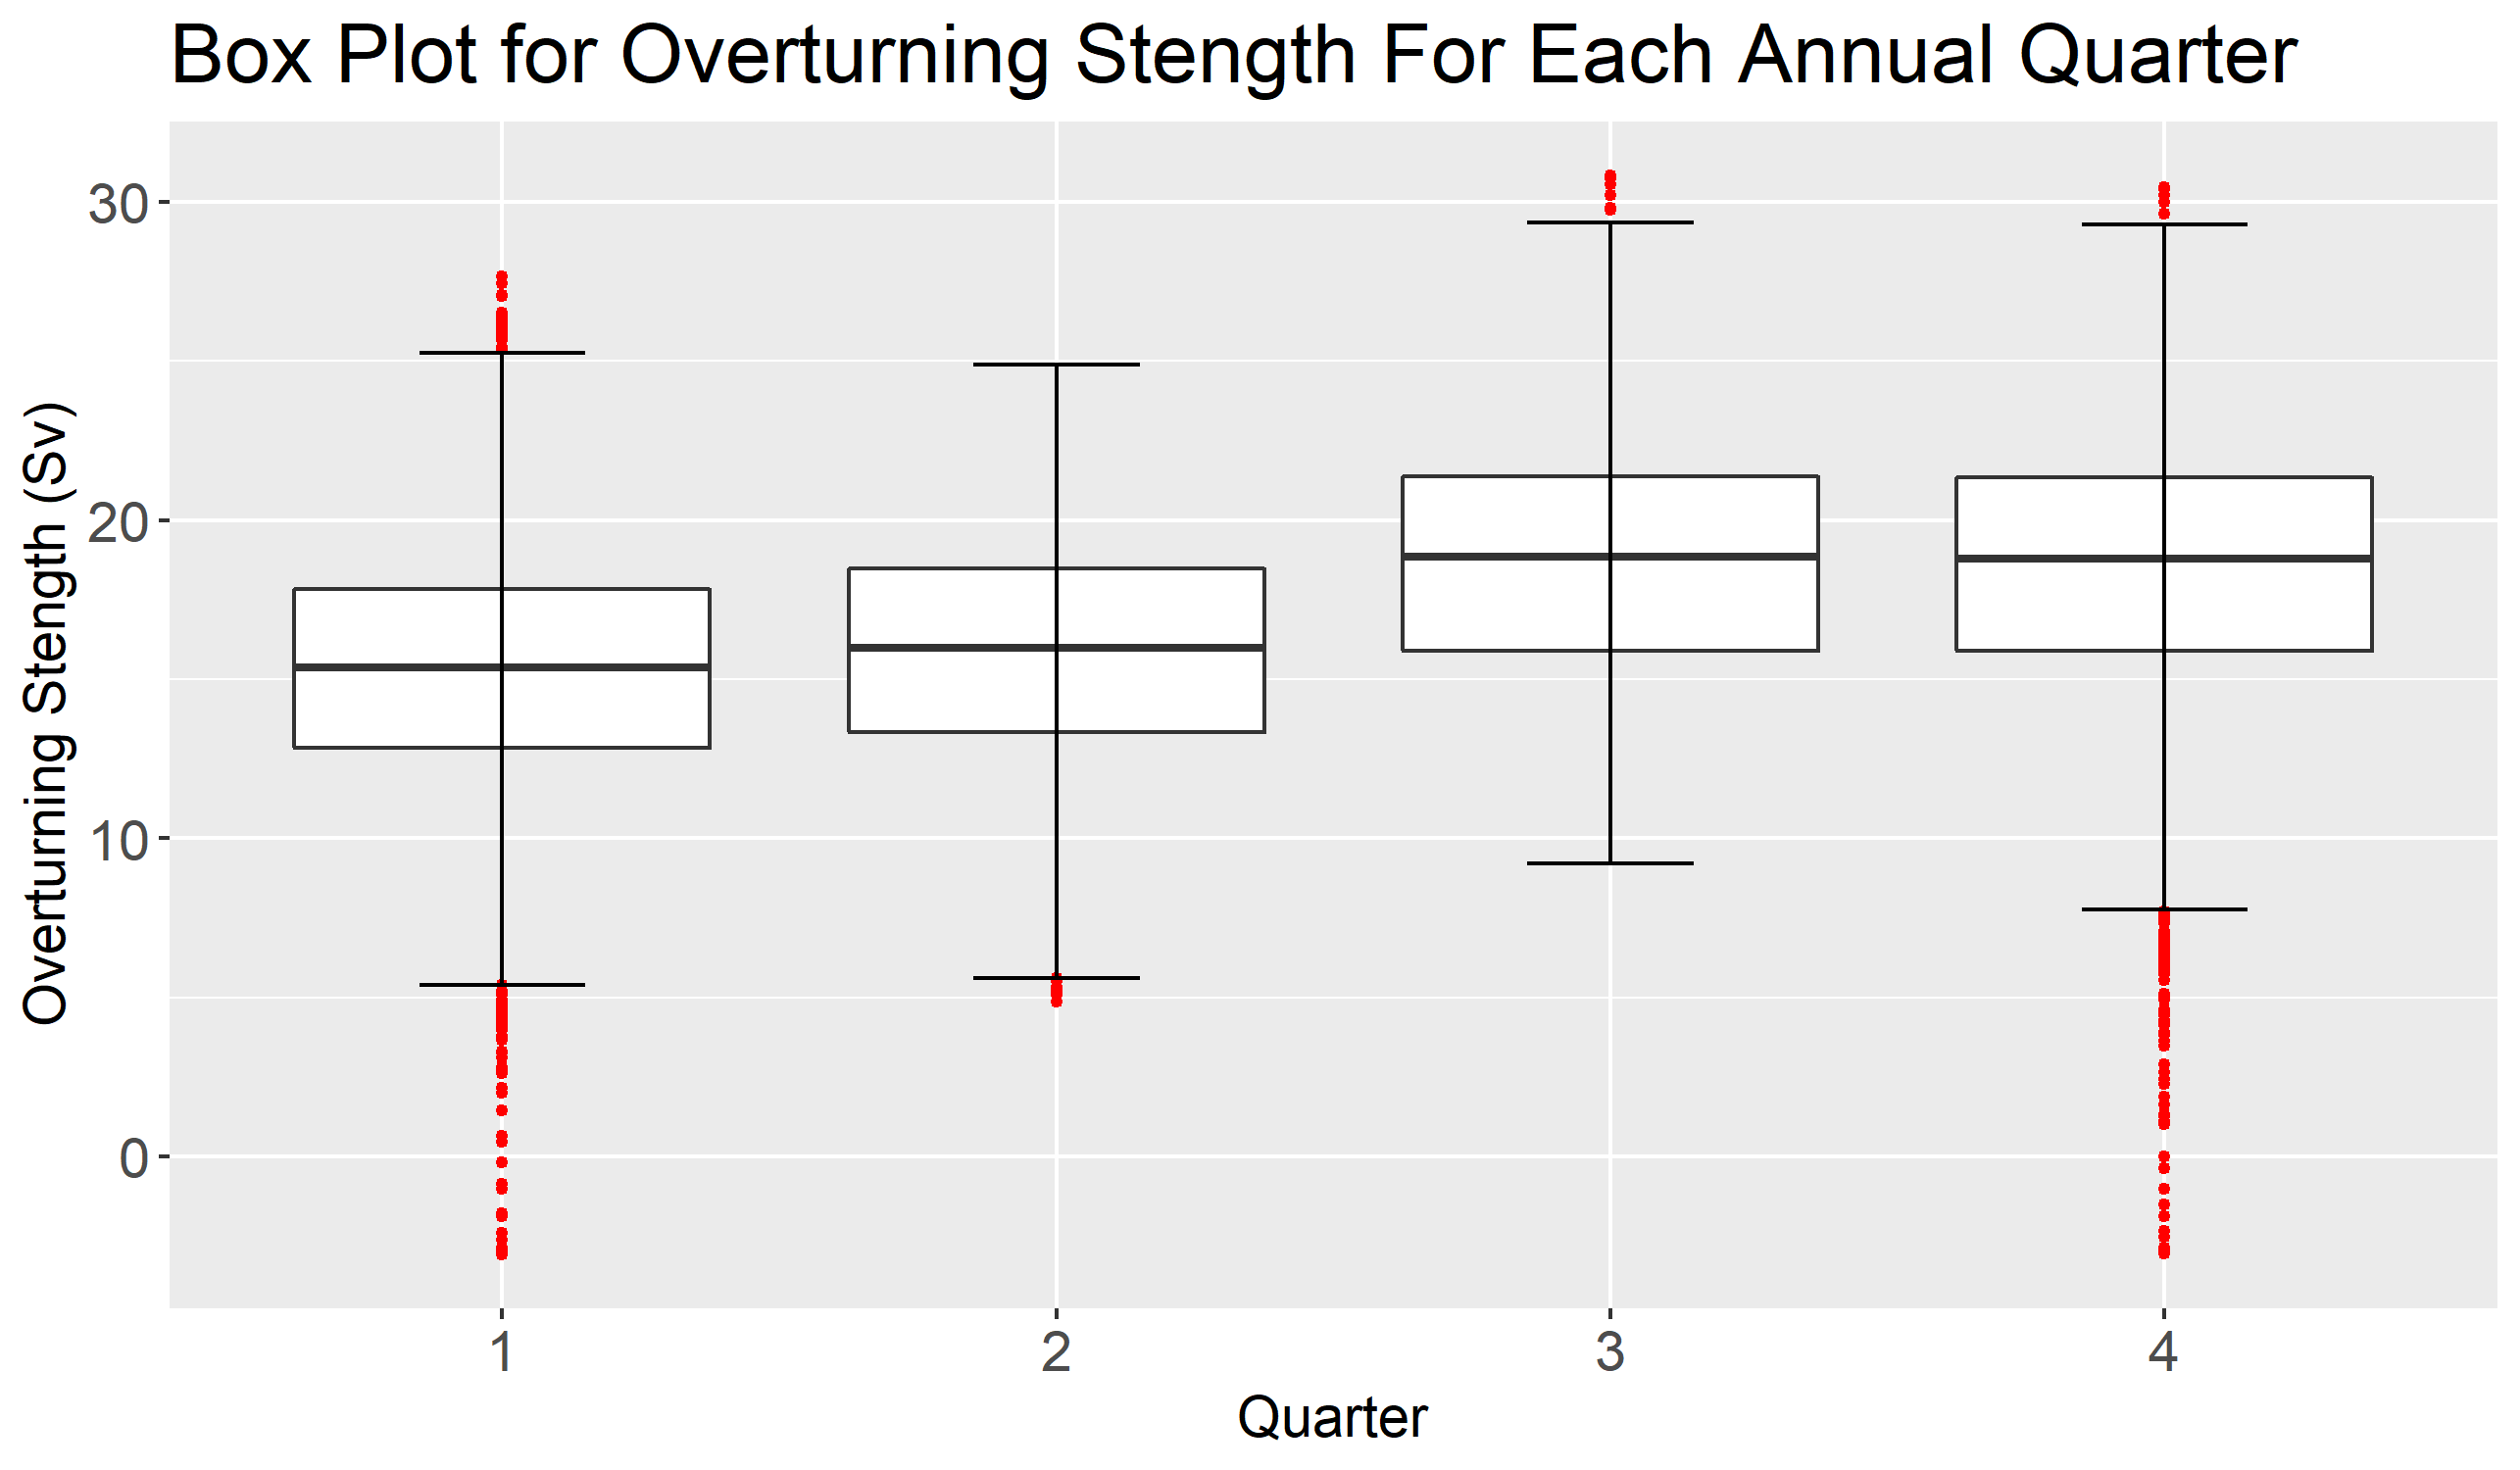
\includegraphics[width=\textwidth]{Sections/DataIntegretity/Plots/Box(yr).png}
        \subcaption{Data grouped into annual quarters.}
    \end{subfigure}
    \begin{subfigure}[b]{\sOneSize\textwidth}
        \centering
        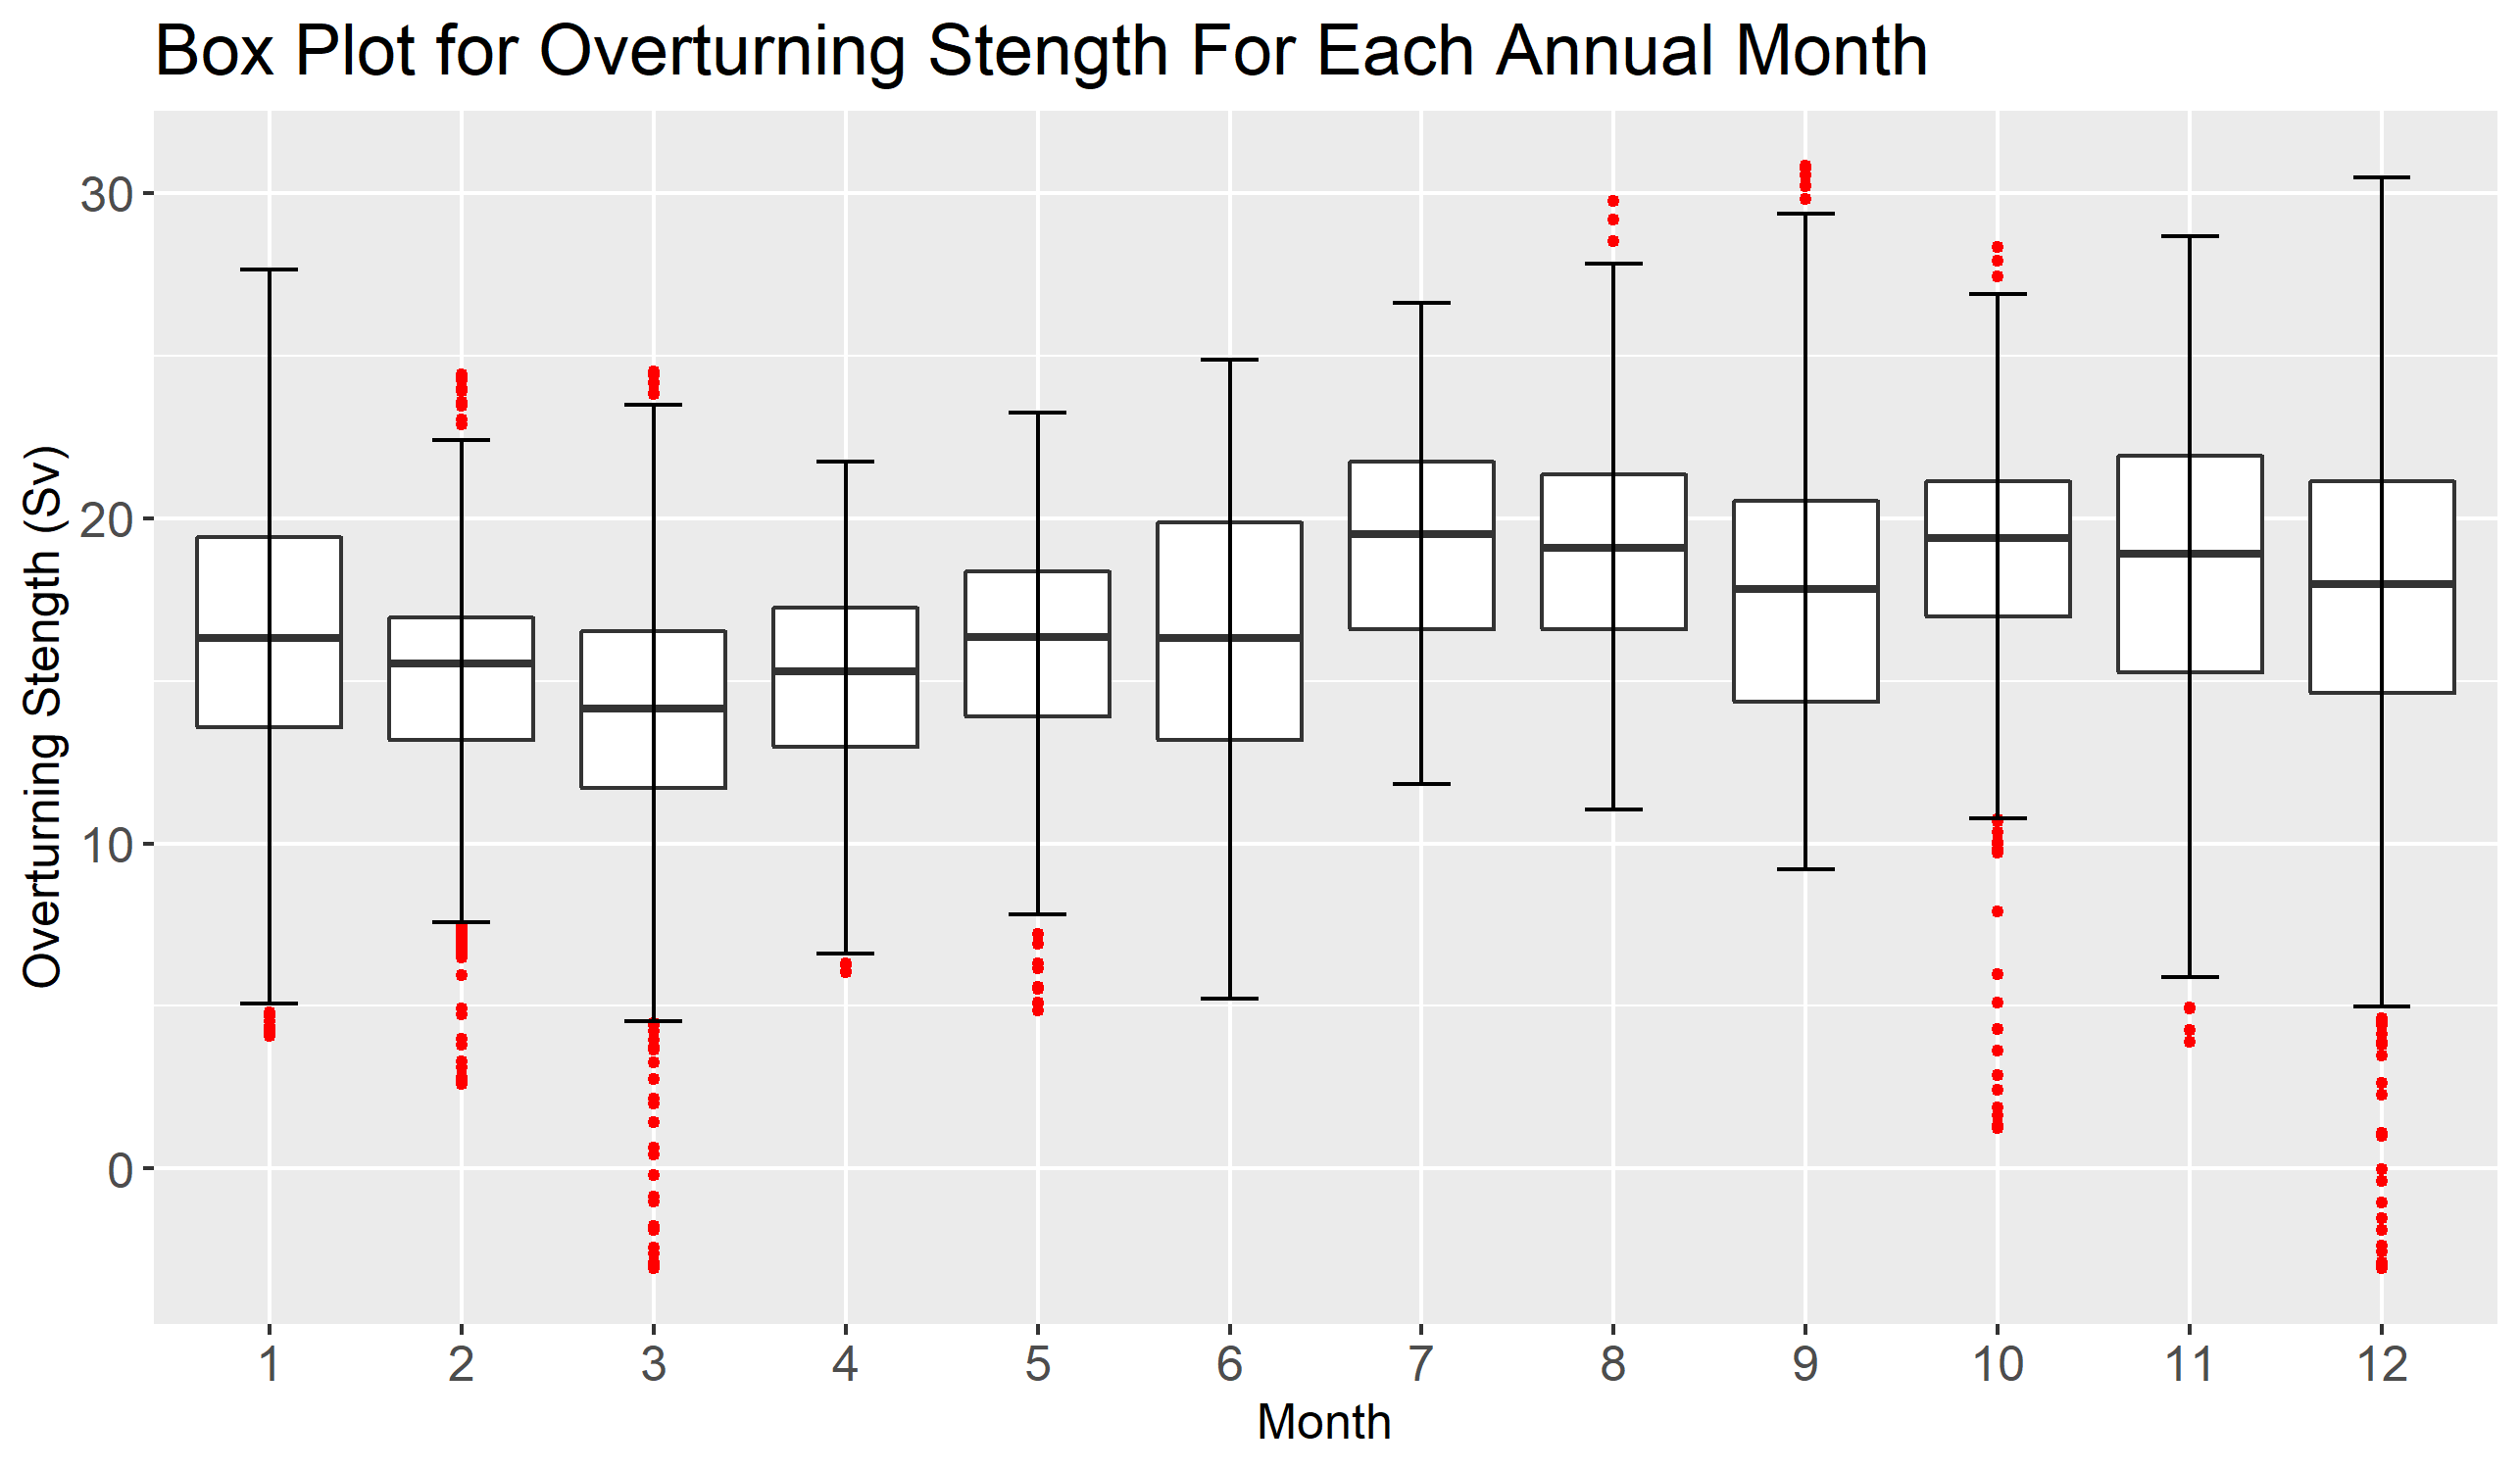
\includegraphics[width=\textwidth]{Sections/DataIntegretity/Plots/Box(mnth).png}
        \subcaption{Data grouped into annual months.}
    \end{subfigure}
\caption{Box plot showing the distribution of overturning strength (Sv) for both annual quarters and for each month. Outliers defined as $\frac{3}{2}\IQR$ from the upper or lower quartiles are highlighted in red.}\label{S1fig:boxplot(yr)}
\end{figure}
We can see in \autoref{S1fig:boxplot(yr)} which uses the interquartile range as a method to detect outliers we find an extremely high number of outliers especially in the first and fourth quartile. To investigate further into these outliers we can extract them from our data and plot them against time.
\nline
Looking at \autoref{S1fig:outliers.ts} we can see that the outliers tend to be grouped together but are spread well throughout the data. We may then conclude that these outliers are instead byproducts of the complex nature and long term trends of the ocean.

\begin{figure}[H]
    \centering
    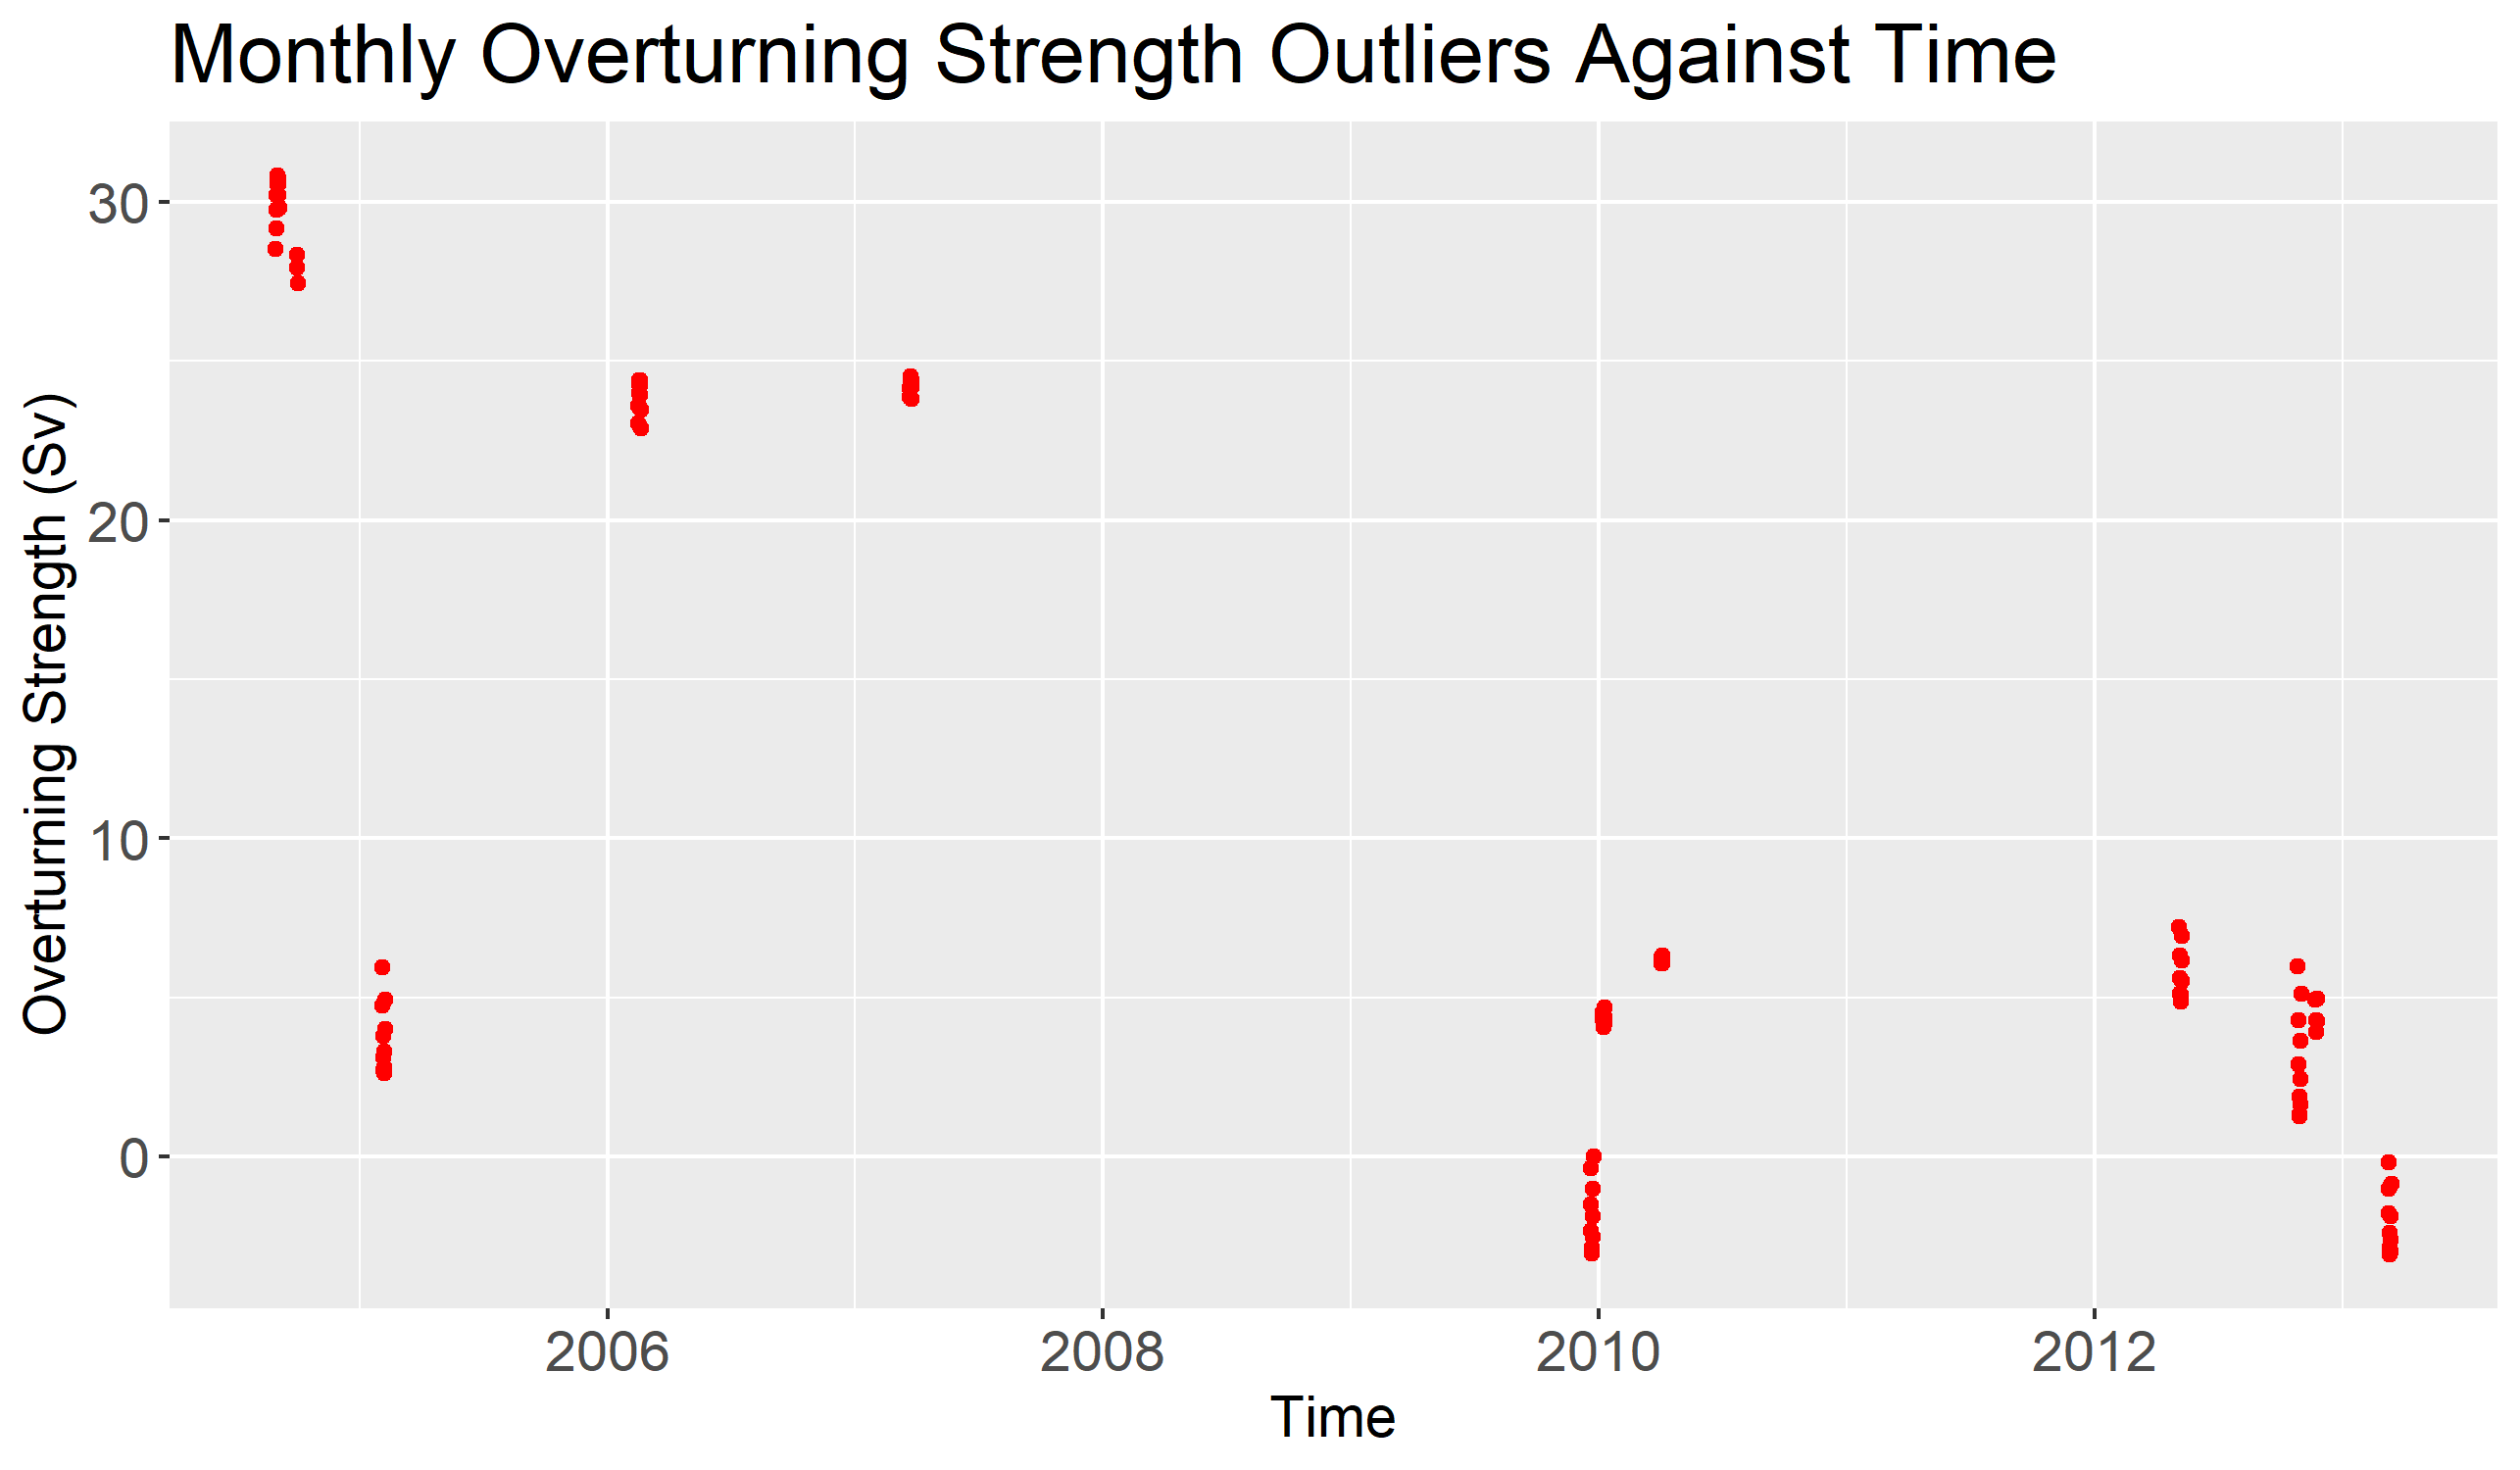
\includegraphics[width=\sOneSize\textwidth]{Sections/DataIntegretity/Plots/outliers.png}
    \caption{Monthly overturning strength outliers plotted against time.}
    \label{S1fig:outliers.ts}
\end{figure}

To get an overview of our data we begin by grouping it into years and annual quarters and then take the mean of each group. This is to reduce noise in our data and also reduces the number of points which helps speeds up the model building computation. We can see this data as a time series in \autoref{S2fig:orig.ts}.

\begin{figure}[H]
    \centering
    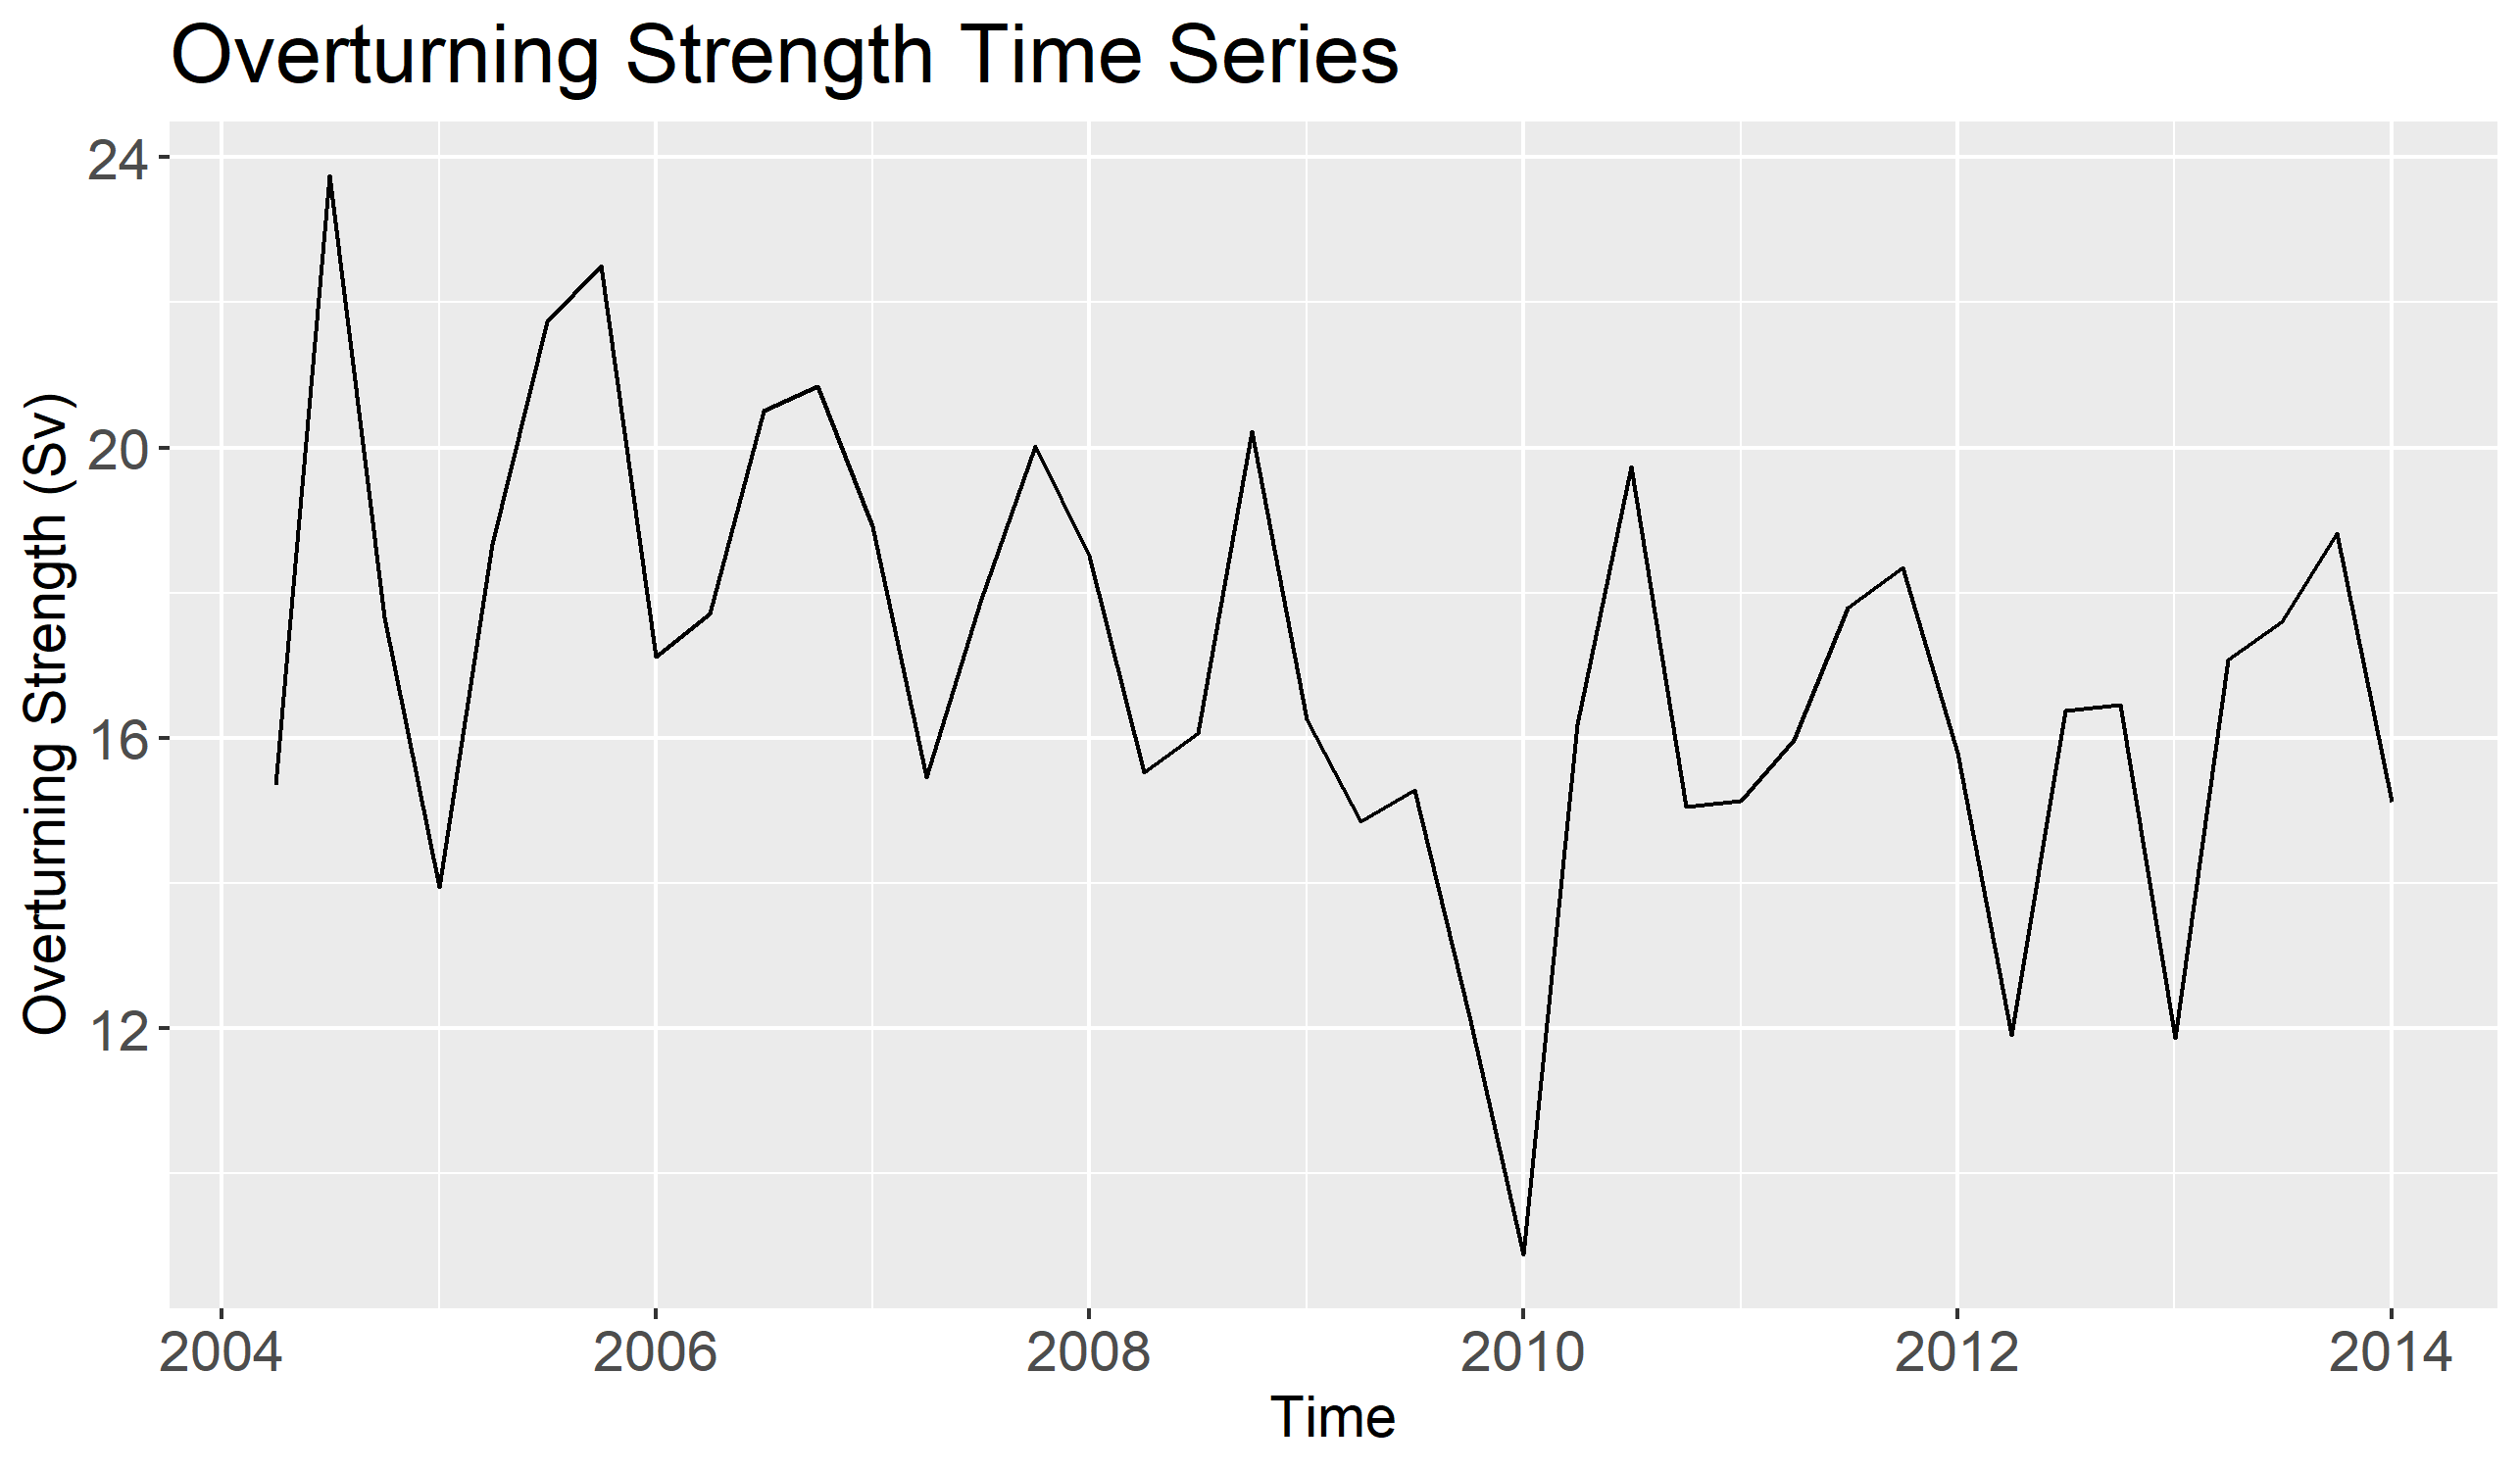
\includegraphics[width=\sOneSize\textwidth]{Sections/DataIntegretity/Plots/orig.png}
    \caption{A time series of our original data where each point is the mean taken over the annual quarter.}
    \label{S2fig:orig.ts}
\end{figure}

Taking a look at \autoref{S2fig:orig.ts} we can see that there appears to be a pattern of changing between up and down within fairly consistent values roughly every half of year. However, this pattern is not followed between 2009 and 2011 when we see a drop shortly followed by another drop before a very sharp upwards tick till halfway through 2010. Whilst this significant drop may seem as an outlier it is generally accepted in the literature, and its origin is uncertain \cite{reduction.cite}.
\nline
With this quick assessment of the data concluding that there are no outliers, we will then continue to build our models without removing any data from the provided data set.
% !TeX root = ..\..\main.tex
\section{ARMA and ARIMA Model}

The first step in building an autoregressive (integrated) moving average (AR(I)MA) model is to determine which process best describes our data. Our process is considered to consist of:

\begin{multicols}{3}
    Autoregressive:
    \begin{equation*}
        \AR{p}: x_t = \sum_{i=1}^p\alpha_ix_{t-i} + \epsilon_t
    \end{equation*}
    \vfill
    \columnbreak
    \noindent Integrated: d is the degree of differencing (the number of times the data have had past values subtracted).
    \vfill
    \columnbreak
    Moving Average:
    \begin{equation*}
        \MA{q}: x_t = \sum_{i=0}^q\beta_i\epsilon_{t-i}
    \end{equation*}
    \vfill
    \columnbreak
\end{multicols}

Where $x_t$ represents the value measured at the $t^{\text{th}}$ time step ($\Delta t$) and $\epsilon_t$ are identical and independent realizations from a normal (Gaussian) distribution with zero mean and variance $\sigma^2$. 

\subsection{Autoregressive Moving Average Model (ARMA)}

An ARMA model only consist off the $\AR{p}$ and $\MA{q}$ often referred to as $\ARMA{p}{q}$ but is identical to \break$\ARIMA{p}{0}{q}$, expressed mathematically as:

\begin{equation*}
   \ARMA{p}{q} : x_t  = \sum_{i=1}^p\alpha_ix_{t-i} + \sum_{i=0}^q\beta_i\epsilon_{t-i} \quad \text{where } \epsilon_t \sim \text{N}\left(0, \sigma^2\right)
\end{equation*}

Our problem then is to fit parameters $(p,q)$ that best describe the underlying process of data.

\subsubsection{Finding optimal parameters}

It is possible that our data may have one of the parameters equal 0 meaning that we just an AR or MA process. One way to check this is to calculate both the auto correlation (ACF) and partial auto correlation functions (PACF). Then using the table below we can see if our data satisfies the criteria.
\par\medskip
\begin{center}
    \begin{tabular}{c|c|c|c}
        & AR(p) & MA(q) & ARMA(p,q) \\
        \hline ACF & Tails off & Cuts off after lag $q$ & Tails off \\
        PACF & Cuts off after lag $p$ & Tails off & Tails off \\
    \end{tabular}
\end{center}
\par\medskip
The ACF and PACF functions of our data is shown in \autoref{S2fig:ACFPACF}. Taking a look at the ACF \autoref{S2fig:ACF} we see that we have two peaks at 0.25 and 1.00 (excluding peak at 0). Then looking at the PACF \autoref{S2fig:PACF} we have one peak at 0.75 but also one peak just below the 95\% confidence interval at 0.25. Since any of these peaks could be down to noise, it is hard to exactly determine our parameters from this analysis alone.

\begin{figure}[H]
    \centering
    \begin{subfigure}[b]{\sOneSize\textwidth}
        \centering
        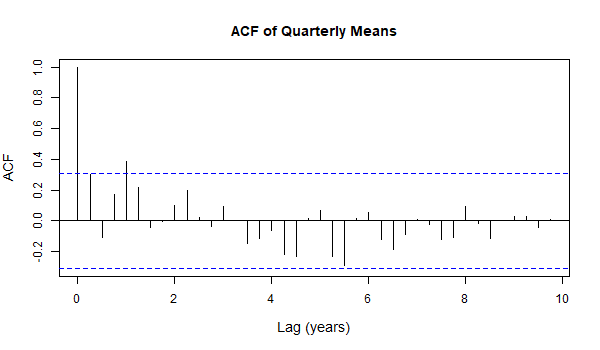
\includegraphics[width=\textwidth]{Sections/ARIMA/Plots/ACF.png}
        \subcaption{Auto correlation function}\label{S2fig:ACF}
    \end{subfigure}
    \begin{subfigure}[b]{\sOneSize\textwidth}
        \centering
        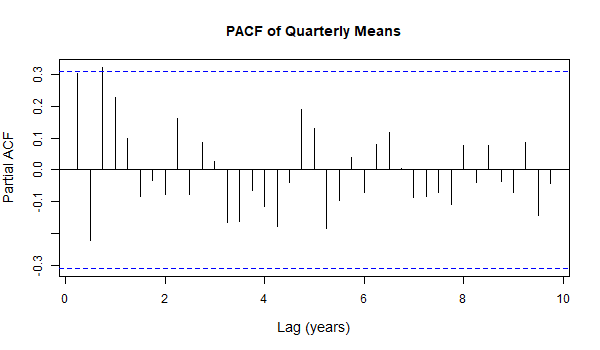
\includegraphics[width=\textwidth]{Sections/ARIMA/Plots/PACF.png}
        \subcaption{Partial auto correlation function}\label{S2fig:PACF}
    \end{subfigure}
\caption{Auto correlation and partial auto correlation functions of our quarterly means data plotted for different lag values in years, with 95\% significance level shown in blue.}
\label{S2fig:ACFPACF}
\end{figure}

We will fit several ARMA models for varying values, $(p,q) \in [0,3]\times[0,7]$ and calculate both the AIC and BIC of the fit. This produces the following results:

\begin{table}[H]
    \begin{center}
        \csvautotabular{S2Tab1.csv}
    \end{center}
    \caption{Sum of AIC and BIC for different $(p,q)$ pairs. For $q > 7$ or $p > 3$ the parameter pair approach the end of the stationarity region.}
    \label{S2:tab_sum}
\end{table}

\begin{itemize}
    \item \input{Sections/ARIMA/Outputs/min1.txt}
    \item \input{Sections/ARIMA/Outputs/min2.txt}
    \item \input{Sections/ARIMA/Outputs/min3.txt}
\end{itemize}

It is worth mentioning that the models allowed for there to be a mean and the best fit was calculated by first using conditional-sum-of-squares to find starting values, then maximum likelihood.
\nline
Continuing with $p = 0$ and $q=1$, we shall take the residuals of our model and produce the following plots:

\begin{figure}[H]
    \centering
    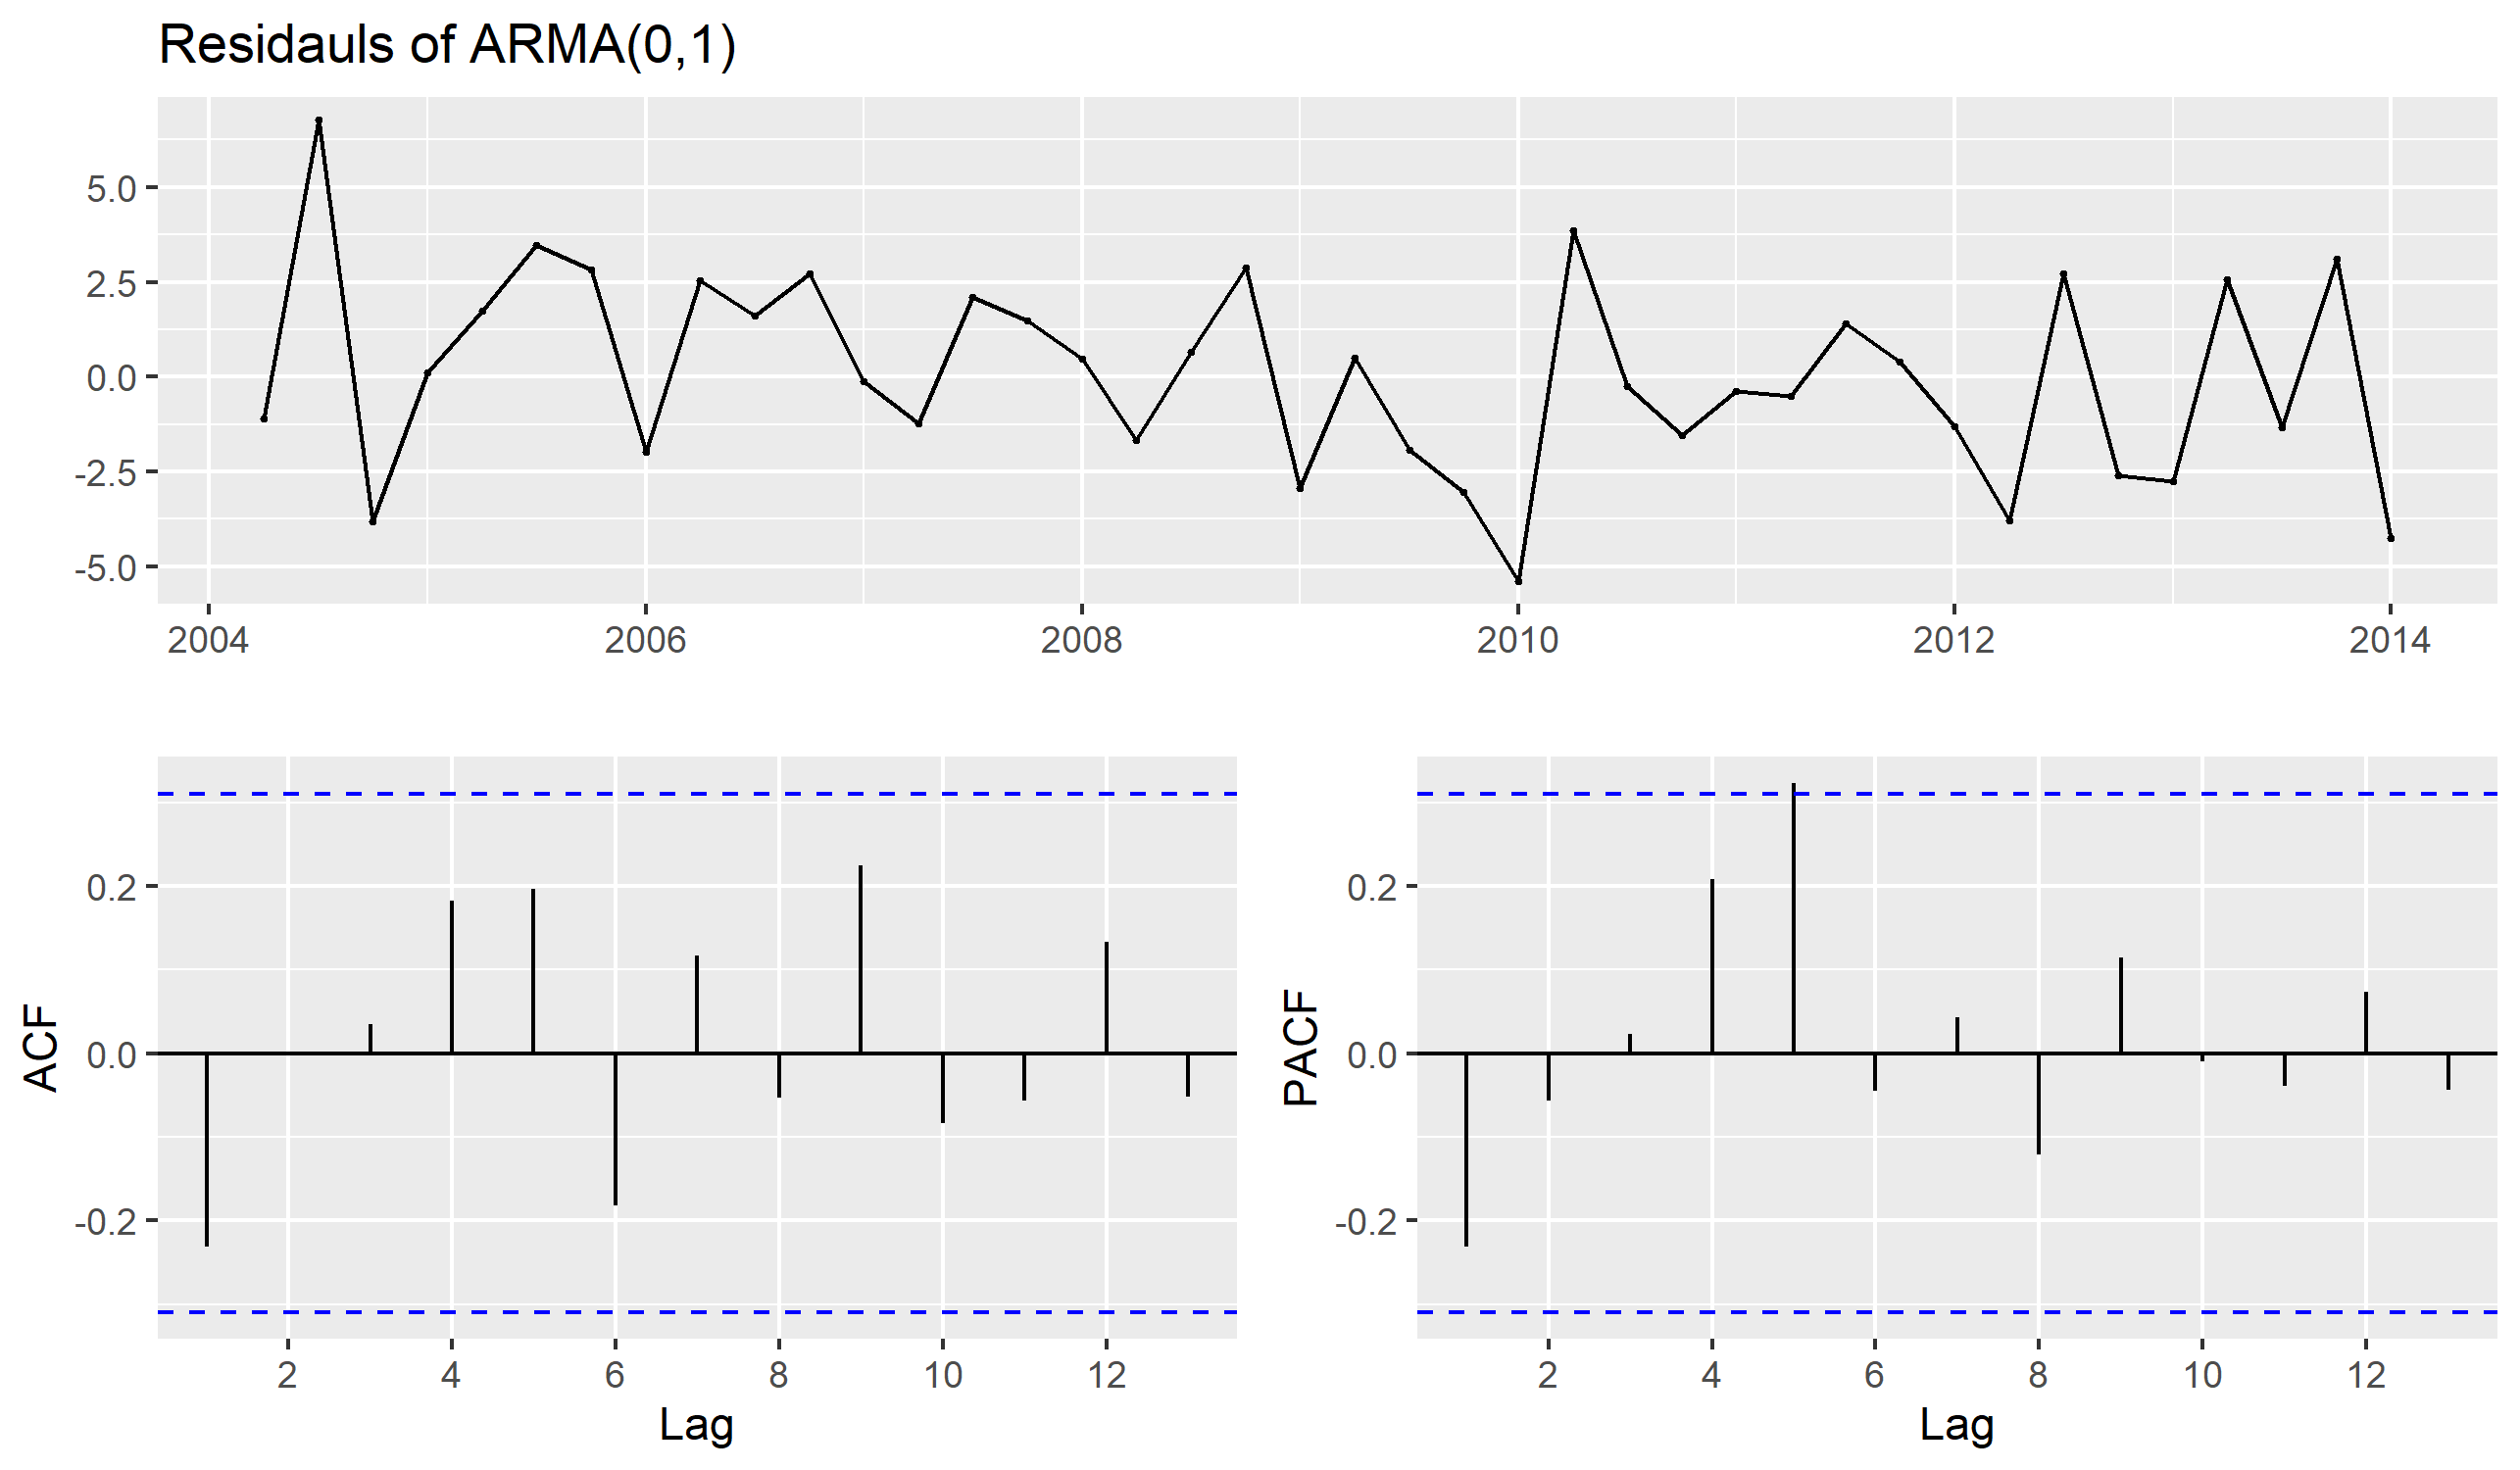
\includegraphics[width=0.75\textwidth]{Sections/ARIMA/Plots/manual_res.png}
    \caption{Residuals from our $\ARMA{0}{1}$ and their ACF and PACF.}
    \label{S2fig:manual_res}
\end{figure}

% \begingroup
% \RaggedRight
\bibliographystyle{alpha}
\bibliography{mybibliography.bib}
% \endgroup

%\appendix
\gdef\thesection{Appendix \Alph{section}:}
\section{R Code}

All files can be found: \small{\url{https://github.com/leele2/Statistcial-Modelling-in-Space-and-Time-CW2/tree/master/RFiles}}

\lstinputlisting[style = R]{../../RFiles/Master.R}

\lstinputlisting[style = R]{../../RFiles/Read_data.R}

\lstinputlisting[style = R]{../../RFiles/Validate.R}

\lstinputlisting[style = R]{../../RFiles/ARMA.R}

\lstinputlisting[style = R]{../../RFiles/DLM.R}

\end{document}